\documentclass[11pt,letterpaper,titlepage]{article}

\usepackage{geometry}
\geometry{left=2cm,right=2cm,top=2cm,bottom=3cm}

\usepackage{setspace}
\onehalfspacing

\usepackage{multicol}
\setlength{\columnsep}{3em}

\usepackage{booktabs}

\usepackage[table,x11names]{xcolor}

\usepackage{multirow}

\usepackage{pgfgantt}

\usepackage{listings}

\usepackage{xcolor}
\definecolor{vgreen}{RGB}{104,180,104}
\definecolor{vblue}{RGB}{49,49,255}
\definecolor{vorange}{RGB}{255,143,102}

\lstdefinestyle{C-style}
{
    language=C,
    basicstyle=\small\ttfamily,
    keywordstyle=\color{vblue},
    identifierstyle=\color{black},
    commentstyle=\color{vgreen},
    % numbers=left,
    numberstyle=\tiny\color{black},
    numbersep=11pt,
    tabsize=4,
    moredelim=*[s][\colorIndex]{[}{]},
    literate=*{:}{:}1
}

\lstdefinestyle{txt-style}
{
    basicstyle=\small\ttfamily,
    % numbers=left,
    numbersep=11pt,
    tabsize=4,
    moredelim=*[s][\colorIndex]{[}{]},
    literate=*{:}{:}1
}

\usepackage{tikz}
\usetikzlibrary{shapes.geometric, arrows, positioning, fit,calc}
\newcommand*\circled[1]{\tikz[baseline=(char.base)]{
            \node[shape=circle,draw,inner sep=1pt] (char) {#1};}}
            
\usepackage{hyperref}
\hypersetup{
    colorlinks,
    citecolor=black,
    filecolor=black,
    linkcolor=black,
    urlcolor=black
}

\usepackage{pifont}

\usepackage[toc,page]{appendix}

\pagestyle{empty}
\usepackage{tikz}
\usetikzlibrary{shapes.geometric, arrows}

\usetikzlibrary{mindmap,trees}
\usepackage{verbatim}

\usepackage{indentfirst}
\setlength{\parindent}{2em}

\usepackage{listings}

\usepackage{chngcntr}
\counterwithin{section}{part}
\renewcommand\thesection{\arabic{section}}

\usepackage{graphicx}

\usepackage{subcaption}

\usepackage{fancyhdr}

\pagestyle{fancy}
\lhead{}
\rhead{}
\lfoot{ECEN 749 Section 601 Lab 6}
\cfoot{\thepage}
\rfoot{@Lei Wang (Wilson)}
\renewcommand{\headrulewidth}{0pt}
\renewcommand{\headwidth}{\textwidth}
\renewcommand{\footrulewidth}{0.4pt}
\newcommand{\RomanNumeralCaps}[1]
    {\MakeUppercase{\romannumeral #1}}

\makeatletter
\newcommand*\@lbracket{[}
\newcommand*\@rbracket{]}
\newcommand*\@colon{:}
\newcommand*\colorIndex{%
    \edef\@temp{\the\lst@token}%
    \ifx\@temp\@lbracket \color{black}%
    \else\ifx\@temp\@rbracket \color{black}%
    \else\ifx\@temp\@colon \color{black}%
    \else \color{vorange}%
    \fi\fi\fi
}
\makeatother

\usepackage{trace}

\begin{document}

\begin{titlepage}
  \centering
	{\scshape\large Texas A\&M University \par}
	\vspace{1cm}
	{\scshape\Large Department of Electrical and Computer Engineering \par}
	\vspace{4cm}
    \vspace{0.5cm}
	{\huge\bfseries ECEN 749 Microprocessor System Design\par}
	\vspace{4cm}
	{\Large Lab 6 Report (Section 601)\par}
	\vspace{1cm}
	{\Large Student: Lei Wang (Wilson)\par}
	\vspace{1cm}
	{\Large UIN: 829009485\par}
	\vspace{1cm}
	{\Large Instructor: Dr. Paul V. Gratz\par}
	\vspace{4cm}
	\vfill

  % Bottom of the page
	{\large Submitted: March 3rd, 2020 \par}

\end{titlepage}

\newpage

\tableofcontents{}

\newpage

\part{Introduction}

Lab 6 aims at creating a character device driver and writing a program to use the hardware multiplier created a few labs before via the character device driver. The character device driver will have 6 functions with the following requirement:

\begin{table}[ht]
\centering
\begin{tabular}{@{}ll@{}}
\toprule
Name            & Requirement                                       \\ \midrule
\texttt{init\_module}    & Map hardware memory address. Register device.     \\ \midrule
\texttt{cleanup\_module} & Unmap hardware memory address. Unregister device. \\ \midrule
\texttt{device\_open}    & Prompt user device is opened.                     \\ \midrule
\texttt{device\_release} & Prompt user device is closed.                     \\ \midrule
\texttt{device\_read}    & Return hardware processing result.                \\ \midrule
\texttt{device\_write}   & Send user input to hardware memory address.       \\ \bottomrule
\end{tabular}
\caption{Functions to be implemented in the character device driver.}
\end{table}

\part{Procedure}

\begin{enumerate}
    
    \item Character device driver:
    
    \begin{enumerate}
        
        \item In the \textbf{lab5b} directory, create a file called \textbf{multiplier.c}. Copy the content in appendix \ref{appendix:sourcecode_multiplier} into the file.
        
        \item Modify the content in the \textbf{Makefile} to the one in appendix \ref{appendix:makefile}.
        
        \item To compile the character device driver, run:
        
        \verb|make ARCH=arm CROSS_COMPILE=arm-xilinx-linux-gnueabi-|
        
        \item Copy the generated file to the micro-SD card. Boot Linux and load the compiled module.
        
    \end{enumerate}
    
    \item C program:
    
    \begin{enumerate}
        
        \item Create a file called \textbf{devtest.c}. Copy the content in appendix \ref{appendix:sourcecode_devtest}
        
        \item To compile the program, run:
        
        \verb|arm-xilinx-linux-gnueabi-gcc -o devtest devtest.c|
        
        \item Copy the compiled program to the micro-SD card. Run \verb|./devtest| in Picocom to test the program.
        
    \end{enumerate}
    
\end{enumerate}

\newpage

\part{Results}

After running

\verb|insmod multiplier.ko|

\verb|mknod /dev/multiplier c 245 0|

\verb|./devtest|

\begin{figure}[ht]
    \centering
    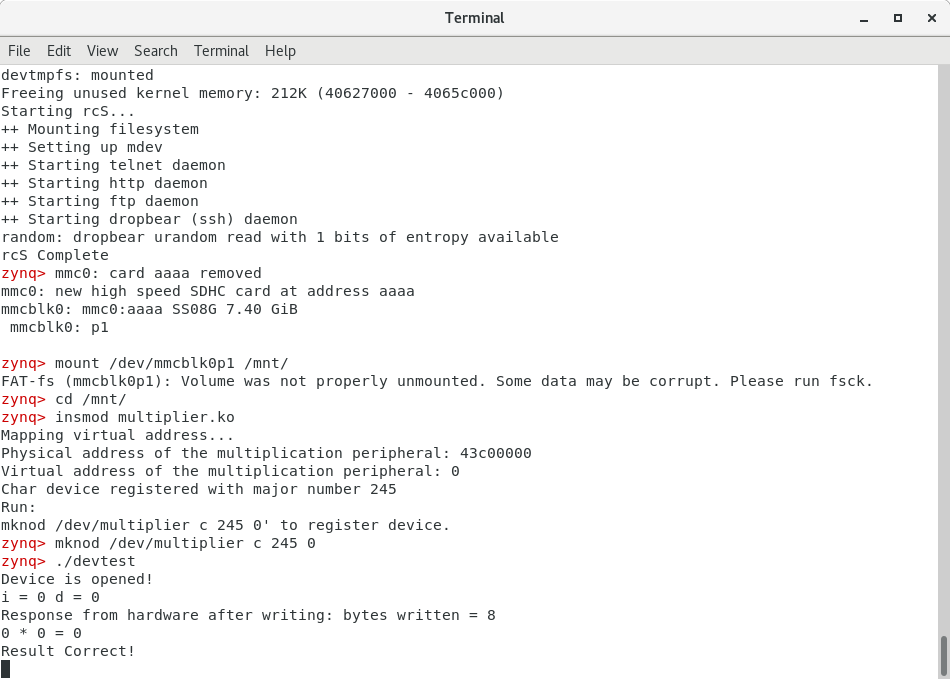
\includegraphics[width=\textwidth]{Register.png}
    \caption{Running the program after 3 lines of commands.}
\end{figure}

\newpage

\begin{figure}[h!]
    \centering
    \begin{subfigure}[b]{0.49\textwidth}
    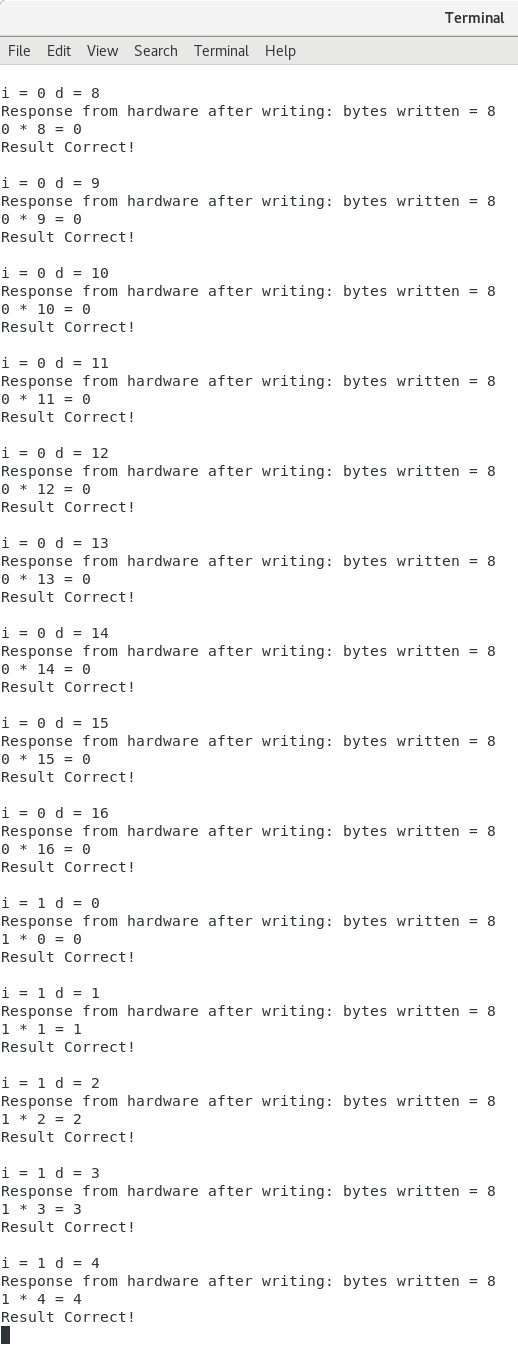
\includegraphics[width=0.9\textwidth]{1.png}
    \caption{Running the program.}
    \end{subfigure}
    \begin{subfigure}[b]{0.49\textwidth}
    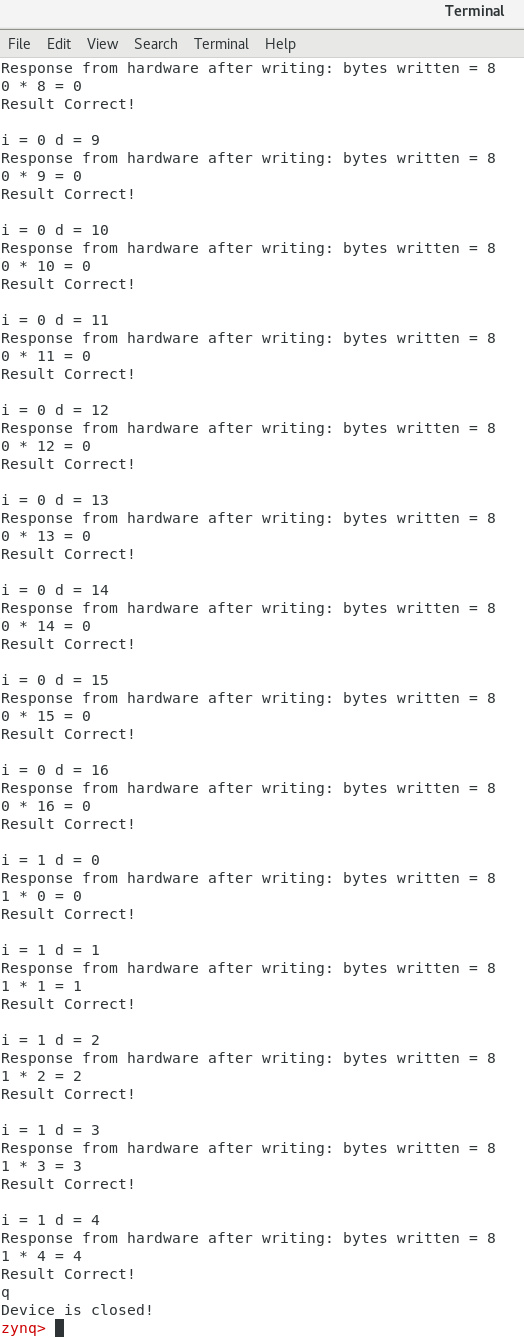
\includegraphics[width=0.9\textwidth]{Close.png}
    \caption{Close the program.}
    \end{subfigure}
    \caption{Program output.}
\end{figure}

To interrupt the program, press q.

\newpage

\part{Conclusion}

As mentioned in the introduction of the report, the hardware multiplier device driver has 6 functions. The device driver is loaded into the Linux kernel the same way as other kernel modules. In lab6, the driver is characterized as a character device driver since it handles data in characters, i.e. 8 bytes. Hence when writing program, always remember to convert input to 8 bytes of continuous data. Different data types such as integers or floats can take multiple bytes of space and to convert such kind of data to character array, type casting may be necessary. A straightforward way is to load the same chunk of data, i.e. a 12-byte-long character array, into an integer array that has three numbers, by using pointers.

The device driver is presented to the user in the form of a file. Hence conventional commands like \texttt{open} or \texttt{close} can be used to handle tasks like write to or read from the hardware.

\textbf{Q: Given that the multiplier hardware uses memory mapped I/O (the processor communicates with
it through explicitly mapped physical addresses), why is the ioremap command required?}

A: User program runs in virtual memory when running Linux on the arm processor. ioremap translates the physical address to virtual memory address, allowing the user to read and write from the hardware.

\textbf{Q: Do you expect that the overall (wall clock) time to perform a multiplication would be better in part 3 of this lab or in the original Lab 3 implementation? Why?}

A: The implementation in lab 6 is expected to take longer time to handle multiplication compared with the one in lab 3. The implementation in lab 3 does not need Linux or a hardware driver. The program communicates with hardware directly. In lab 6, the program talks to the driver first and then the driver communicates with the hardware. Hence it takes longer.

\textbf{Q: Contrast the approach in this lab with that of Lab 3. What are the benefits and costs associated with each approach?}

A: Lab 3 requires less hardware resource and does not use the ARM processor. Lab 6 uses more hardware resource and needs the ARM processor. Using the ARM processor supports booting Linux. Under the Linux environment, user program does not need to communicate with the low-level hardware directly but with the hardware driver. The driver provides a layer of abstraction and makes the program easier to write and safer to run. However, a hardware driver and other setup measures are needed to run program under Linux. Lab 3 can be a straightforward implementation but it lacks support for peripherals such as the micro-SD card or USB devices. By using Linux, not only the program is easier to write but support for peripheral devices is made possible. Though performance may be degraded due to overhead such as the hardware driver or higher hardware resource usage.

\textbf{Q: Explain why it is important that the device registration is the last thing that is done in the initialization routine of a device driver. Likewise, explain why un-registering a device must happen first in the exit routine of a device driver.}

A: By registering, program can have access the device. To prevent errors such as accessing an invalid memory address, the hardware memory address mapping must be done prior to registration. By placing the un-registering process before the exit routine, when program has access to the device, the access always has a valid memory address. When the device is not accessible, before the exit routing, the device memory address is still valid.

\newpage

\begin{appendices}

\section{Makefile}
\label{appendix:makefile}
\lstinputlisting[style={txt-style}]{Makefile}

\section{multiplier.c}
\label{appendix:sourcecode_multiplier}
\lstinputlisting[style={txt-style}]{multiplier.c}

\section{devtest.c}
\label{appendix:sourcecode_devtest}
\lstinputlisting[style={txt-style}]{devtest.c}

\end{appendices}

\end{document}
